\documentclass{standalone}
\usepackage{tikz}
\usetikzlibrary{patterns, positioning}


\begin{document}
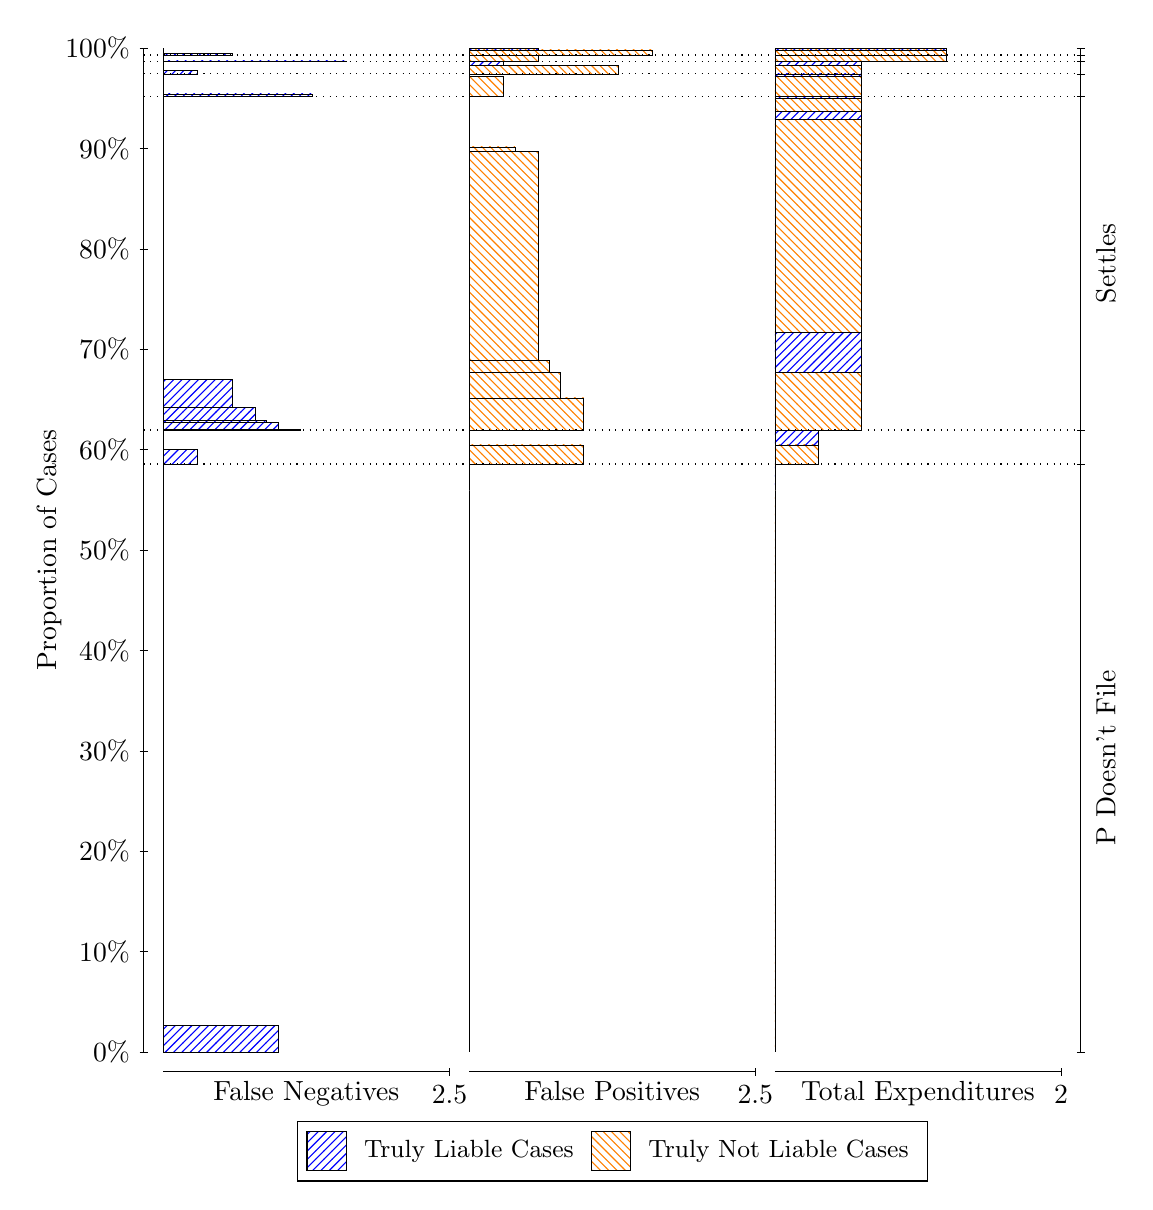
\begin{tikzpicture}
\draw[black, very thin] (1.5,1.75) -- (1.5,14.5);
\node[rotate=90, text=black, anchor=center] at (0.3, 8.125) {Proportion of Cases};
\draw[black, very thin] (1.45,1.75) -- (1.55,1.75);
\node[text=black, anchor=east] at (1.45, 1.75) {0\%};
\draw[black, very thin] (1.45,3.025) -- (1.55,3.025);
\node[text=black, anchor=east] at (1.45, 3.025) {10\%};
\draw[black, very thin] (1.45,4.3) -- (1.55,4.3);
\node[text=black, anchor=east] at (1.45, 4.3) {20\%};
\draw[black, very thin] (1.45,5.575) -- (1.55,5.575);
\node[text=black, anchor=east] at (1.45, 5.575) {30\%};
\draw[black, very thin] (1.45,6.85) -- (1.55,6.85);
\node[text=black, anchor=east] at (1.45, 6.85) {40\%};
\draw[black, very thin] (1.45,8.125) -- (1.55,8.125);
\node[text=black, anchor=east] at (1.45, 8.125) {50\%};
\draw[black, very thin] (1.45,9.4) -- (1.55,9.4);
\node[text=black, anchor=east] at (1.45, 9.4) {60\%};
\draw[black, very thin] (1.45,10.675) -- (1.55,10.675);
\node[text=black, anchor=east] at (1.45, 10.675) {70\%};
\draw[black, very thin] (1.45,11.95) -- (1.55,11.95);
\node[text=black, anchor=east] at (1.45, 11.95) {80\%};
\draw[black, very thin] (1.45,13.225) -- (1.55,13.225);
\node[text=black, anchor=east] at (1.45, 13.225) {90\%};
\draw[black, very thin] (1.45,14.5) -- (1.55,14.5);
\node[text=black, anchor=east] at (1.45, 14.5) {100\%};

\draw[black, very thin] (13.4,1.75) -- (13.4,14.5);
\draw[black, very thin] (13.35,1.75) -- (13.45,1.75);
\node[anchor=west] at (13.35, 1.75) {};
\draw[black, very thin] (13.35,9.2168) -- (13.45,9.2168);
\node[anchor=west] at (13.35, 9.2168) {};
\draw[black, very thin] (13.35,9.6485) -- (13.45,9.6485);
\node[anchor=west] at (13.35, 9.6485) {};
\draw[black, very thin] (13.35,13.884) -- (13.45,13.884);
\node[anchor=west] at (13.35, 13.884) {};
\draw[black, very thin] (13.35,14.171) -- (13.45,14.171);
\node[anchor=west] at (13.35, 14.171) {};
\draw[black, very thin] (13.35,14.33) -- (13.45,14.33);
\node[anchor=west] at (13.35, 14.33) {};
\draw[black, very thin] (13.35,14.411) -- (13.45,14.411);
\node[anchor=west] at (13.35, 14.411) {};
\draw[black, very thin] (13.35,14.5) -- (13.45,14.5);
\node[anchor=west] at (13.35, 14.5) {};

\draw[black, very thin, pattern color=blue, pattern=north east lines] (1.75,1.75) rectangle (3.2033,2.0844);
\draw[black, very thin, pattern color=orange, pattern=north west lines] (1.75,2.0844) rectangle (1.75,9.2168);
\draw[black, very thin, pattern color=blue, pattern=north east lines] (1.75,9.2168) rectangle (2.186,9.4048);
\draw[black, very thin, pattern color=orange, pattern=north west lines] (1.75,9.4048) rectangle (1.75,9.6485);
\draw[black, very thin, pattern color=blue, pattern=north east lines] (1.75,9.6485) rectangle (3.494,9.6546);
\draw[black, very thin, pattern color=blue, pattern=north east lines] (1.75,9.6546) rectangle (3.2033,9.7479);
\draw[black, very thin, pattern color=blue, pattern=north east lines] (1.75,9.7479) rectangle (3.058,9.7759);
\draw[black, very thin, pattern color=blue, pattern=north east lines] (1.75,9.7759) rectangle (2.9127,9.9388);
\draw[black, very thin, pattern color=blue, pattern=north east lines] (1.75,9.9388) rectangle (2.622,10.287);
\draw[black, very thin, pattern color=orange, pattern=north west lines] (1.75,10.287) rectangle (1.75,13.884);
\draw[black, very thin, pattern color=blue, pattern=north east lines] (1.75,13.884) rectangle (3.6393,13.917);
\draw[black, very thin, pattern color=orange, pattern=north west lines] (1.75,13.917) rectangle (1.75,14.171);
\draw[black, very thin, pattern color=blue, pattern=north east lines] (1.75,14.171) rectangle (2.186,14.22);
\draw[black, very thin, pattern color=orange, pattern=north west lines] (1.75,14.22) rectangle (1.75,14.33);
\draw[black, very thin, pattern color=blue, pattern=north east lines] (1.75,14.33) rectangle (4.0753,14.337);
\draw[black, very thin, pattern color=orange, pattern=north west lines] (1.75,14.337) rectangle (1.75,14.411);
\draw[black, very thin, pattern color=blue, pattern=north east lines] (1.75,14.411) rectangle (2.622,14.436);
\draw[black, very thin, pattern color=orange, pattern=north west lines] (1.75,14.436) rectangle (1.75,14.5);
\draw[black, very thin, pattern color=orange, pattern=north west lines] (5.6333,1.75) rectangle (5.6333,8.8825);
\draw[black, very thin, pattern color=blue, pattern=north east lines] (5.6333,8.8825) rectangle (5.6333,9.2168);
\draw[black, very thin, pattern color=orange, pattern=north west lines] (5.6333,9.2168) rectangle (7.0867,9.4605);
\draw[black, very thin, pattern color=blue, pattern=north east lines] (5.6333,9.4605) rectangle (5.6333,9.6485);
\draw[black, very thin, pattern color=orange, pattern=north west lines] (5.6333,9.6485) rectangle (7.0867,10.056);
\draw[black, very thin, pattern color=orange, pattern=north west lines] (5.6333,10.056) rectangle (6.796,10.38);
\draw[black, very thin, pattern color=orange, pattern=north west lines] (5.6333,10.38) rectangle (6.6507,10.538);
\draw[black, very thin, pattern color=orange, pattern=north west lines] (5.6333,10.538) rectangle (6.5053,13.191);
\draw[black, very thin, pattern color=orange, pattern=north west lines] (5.6333,13.191) rectangle (6.2147,13.245);
\draw[black, very thin, pattern color=blue, pattern=north east lines] (5.6333,13.245) rectangle (5.6333,13.884);
\draw[black, very thin, pattern color=orange, pattern=north west lines] (5.6333,13.884) rectangle (6.0693,14.138);
\draw[black, very thin, pattern color=blue, pattern=north east lines] (5.6333,14.138) rectangle (5.6333,14.171);
\draw[black, very thin, pattern color=orange, pattern=north west lines] (5.6333,14.171) rectangle (7.5227,14.281);
\draw[black, very thin, pattern color=blue, pattern=north east lines] (5.6333,14.281) rectangle (6.0693,14.33);
\draw[black, very thin, pattern color=orange, pattern=north west lines] (5.6333,14.33) rectangle (6.5053,14.404);
\draw[black, very thin, pattern color=blue, pattern=north east lines] (5.6333,14.404) rectangle (5.6333,14.411);
\draw[black, very thin, pattern color=orange, pattern=north west lines] (5.6333,14.411) rectangle (7.9587,14.475);
\draw[black, very thin, pattern color=blue, pattern=north east lines] (5.6333,14.475) rectangle (6.5053,14.5);
\draw[black, very thin, pattern color=orange, pattern=north west lines] (9.5167,1.75) rectangle (9.5167,8.8825);
\draw[black, very thin, pattern color=blue, pattern=north east lines] (9.5167,8.8825) rectangle (9.5167,9.2168);
\draw[black, very thin, pattern color=orange, pattern=north west lines] (9.5167,9.2168) rectangle (10.062,9.4605);
\draw[black, very thin, pattern color=blue, pattern=north east lines] (9.5167,9.4605) rectangle (10.062,9.6485);
\draw[black, very thin, pattern color=orange, pattern=north west lines] (9.5167,9.6485) rectangle (10.607,10.38);
\draw[black, very thin, pattern color=blue, pattern=north east lines] (9.5167,10.38) rectangle (10.607,10.891);
\draw[black, very thin, pattern color=orange, pattern=north west lines] (9.5167,10.891) rectangle (10.607,13.598);
\draw[black, very thin, pattern color=blue, pattern=north east lines] (9.5167,13.598) rectangle (10.607,13.698);
\draw[black, very thin, pattern color=orange, pattern=north west lines] (9.5167,13.698) rectangle (10.607,13.856);
\draw[black, very thin, pattern color=blue, pattern=north east lines] (9.5167,13.856) rectangle (10.607,13.884);
\draw[black, very thin, pattern color=orange, pattern=north west lines] (9.5167,13.884) rectangle (10.607,14.138);
\draw[black, very thin, pattern color=blue, pattern=north east lines] (9.5167,14.138) rectangle (10.607,14.171);
\draw[black, very thin, pattern color=orange, pattern=north west lines] (9.5167,14.171) rectangle (10.607,14.281);
\draw[black, very thin, pattern color=blue, pattern=north east lines] (9.5167,14.281) rectangle (10.607,14.33);
\draw[black, very thin, pattern color=orange, pattern=north west lines] (9.5167,14.33) rectangle (11.697,14.404);
\draw[black, very thin, pattern color=blue, pattern=north east lines] (9.5167,14.404) rectangle (11.697,14.411);
\draw[black, very thin, pattern color=orange, pattern=north west lines] (9.5167,14.411) rectangle (11.697,14.475);
\draw[black, very thin, pattern color=blue, pattern=north east lines] (9.5167,14.475) rectangle (11.697,14.5);
\draw[black, dotted] (1.5,9.2168) -- (13.4,9.2168);
\draw[black, dotted] (1.5,9.6485) -- (13.4,9.6485);
\draw[black, dotted] (1.5,13.884) -- (13.4,13.884);
\draw[black, dotted] (1.5,14.171) -- (13.4,14.171);
\draw[black, dotted] (1.5,14.33) -- (13.4,14.33);
\draw[black, dotted] (1.5,14.411) -- (13.4,14.411);
\draw[black, very thin] (1.75,1.5) -- (5.3833,1.5);
\node[text=black, anchor=north] at (3.5667, 1.5) {False Negatives};
\draw[black, very thin] (5.3833,1.45) -- (5.3833,1.55);
\node[text=black, anchor=north] at (5.3833, 1.45) {2.5};

\draw[black, very thin] (5.6333,1.5) -- (9.2667,1.5);
\node[text=black, anchor=north] at (7.45, 1.5) {False Positives};
\draw[black, very thin] (9.2667,1.45) -- (9.2667,1.55);
\node[text=black, anchor=north] at (9.2667, 1.45) {2.5};

\draw[black, very thin] (9.5167,1.5) -- (13.15,1.5);
\node[text=black, anchor=north] at (11.333, 1.5) {Total Expenditures};
\draw[black, very thin] (13.15,1.45) -- (13.15,1.55);
\node[text=black, anchor=north] at (13.15, 1.45) {2};

\node[text=black, centered, rotate=90] at (13.72, 5.4834) {P Doesn't File};

\node[text=black, centered, rotate=90] at (13.72, 11.766) {Settles};





\draw (7.449999999999999,1.5) node[draw=none] (baseCoordinate) {};
\begin{scope}[align=center]
        \matrix[scale=0.5, draw=black, below=0.5cm of baseCoordinate, nodes={draw}, column sep=0.1cm]{
            \node[rectangle, draw, minimum width=0.5cm, minimum height=0.5cm, pattern color=blue, pattern=north east lines] {}; &
            \node[draw=none, font=\small, text=black] (B) {Truly Liable Cases}; &
            \node[rectangle, draw, minimum width=0.5cm, minimum height=0.5cm, pattern color=orange, pattern=north west lines] {}; &
            \node[draw=none, font=\small, text=black] (B) {Truly Not Liable Cases}; \\
            };
\end{scope}

\end{tikzpicture}
\end{document}